%!TEX root = Thesis.tex
\chapter{Concept}
     The chapter poses and describes a concept of a user-friendly generic frontend for exploring sensor data, 
     through designing a software architecture and a mockup of a web-based user interface that in the same time controlled and provisioned by end users request. The concept is developed based on the analysis of the current state of the art, up-to-date technologies and usability characteristics. According to defined requirements in chapter 2 to the third-party services and applications and knowledge gained from the studied related works (chapter 3), was proposed concept based on 3-tier architecture and in details described in section 4.2 - 4.4.

\section{3-tier Architecture}
Since the concept of a generic frontend should be distributed as much as possible, it is necessary to determine software architecture 
to a 3-tier architecture, in which presentation, application processing, and data management functions are logically separated.
Figure 4.1 shows this architecture:
\begin{itemize}
\item Data Tier: data from different types of sensors
\item Application Tier: registry and proxy
\item Client Tier: web-based UI
\end{itemize} 
\begin{figure}[!ht]
\centering
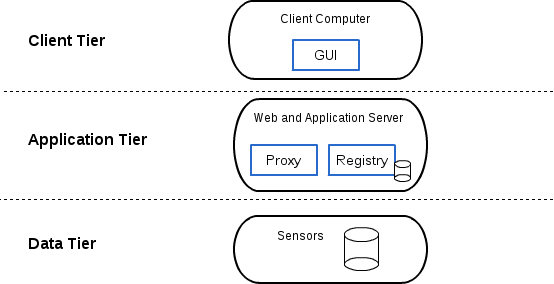
\includegraphics[scale=0.7]{images/3tier.png}   
\caption[3-tier Architecture]{3-tier Architecture}
\label{img:3-tier Architecture}                           
\end{figure}
\emph{Client Tier} hosts the presentation layer components. The main function of the interface is to translate tasks and results to graphical user interface that can be easily understandable and explorable from any kind of device. That satisfy requirements of the usability(section 3.4).
\newline
\emph{Application Tier} includes business logic, logic tier and data access tier. It controls an application's functionality by performing detailed processing, transformation of one type data to another one, defines an interface of interconnection between client tier and data tier.
\newline
\emph{Data Tier} consists source of data that have to be retrieved by application tier to a Client Tier, by request from a end user. This tier keeps data neutral and independent from application server or business logic. Giving data its own tier also improves scalability. 
\newline
The three tiers architecture may seem similar to the model-view-controller (MVC) concept. However, topologically they are different. A fundamental rule in a three tier architecture is the client tier never communicates directly with the data tier; in a three-tier model all communication must pass through the middle tier. Conceptually the three-tier architecture is linear. However, the MVC architecture is triangular: the view sends updates to the controller, the controller updates the model, and the view gets updated directly from the model.
From a historical perspective the three-tier architecture concept emerged in the 1990s from observations of distributed systems (e.g., web applications) where the client, middleware and data tiers ran on physically separate platforms. Today, MVC and similar model-view-presenter (MVP) are Separation of Concerns design patterns that apply exclusively to the presentation layer of a larger system. In simple scenarios MVC may represent the primary design of a system, reaching directly into the database; however, in most scenarios the Controller and Model in MVC have a loose dependency on either a Service or Data layer/tier. This is all about Client-Server architecture.
\newline
In the next section gives an detailed explanation about structure modules in 3-tier architecture.

\section{Client Tier}
  The client tier or another name is presentation tier is a layer which users can access directly such as a web page by using browser. It is the first that user see. This tier consists logic and GUI by using which, user can communicate with sensor in a way that is presented on Figure 4.2. Also Client Tier responsible to be adapted to any kind of mobile or desktop devices that user can use. Therefore as a cross-platforming approach was chosen web-based solution, where all communication flows through the browser.

    \begin{figure}[!ht]
    \centering
    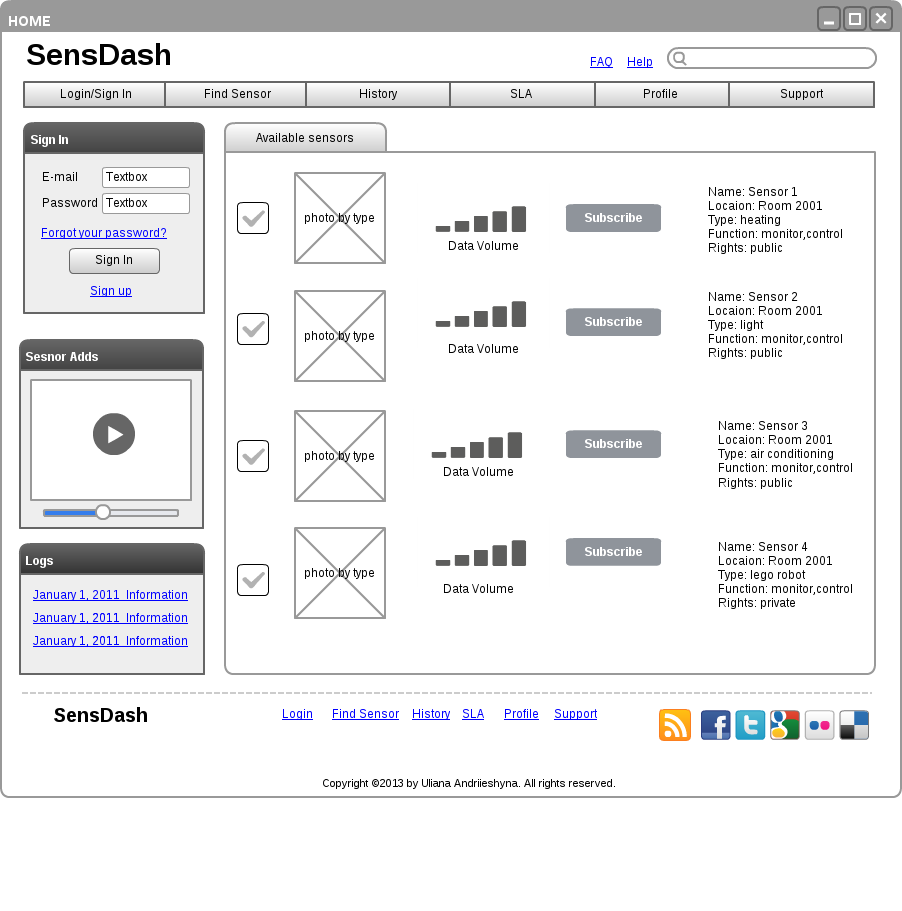
\includegraphics[scale=0.4]{images/Mockup.png}   
    \caption[GUI Mockup]{GUI Mockup}
    \label{img:GUI Mockup}                           
    \end{figure}
    Figure 4.2 presents simple content layout in which user can be interested in. It consists:
      \begin{itemize}
      \item Login form with user name and password fields. After user logged in, the system defines his/her rights and applies visibility rules according to credentials. User that have an admin rights receives an opportunity to control and manipulate sensors. Simple user will receive an opportunity to get a statistic and information from sensors.
      \item Sensor icon defines what is the current type of sensor, e.g. light, temperature, heating, robot lego, etc. In such a way user can easily, even in seconds, understand and catch what is the main function of a sensor in the list.
      \item Availability or unavailability to see alive statistics. User can subscribe only to the available services. If some services become unavailable it will be automatically marked as inactive and after refreshing will be deleted from the list of available sensors and moved to a history tab.
      \item Data Volume icon shows what is the average data stream volume needed to retrieve sensor data(Kb/s). The dashboard should automatically adapt quality of streaming data to necessary and possible bandwidth of available connection(Wi-Fi, 3G, GPRS)
      \end{itemize}
    The common use case from a end-user point of view shown on Figure 4.3. User can use any type of mobile device and his favorite browser to receive information from the sensors by using web-site as a dashboard.

        \begin{figure}[!ht]
        \centering
        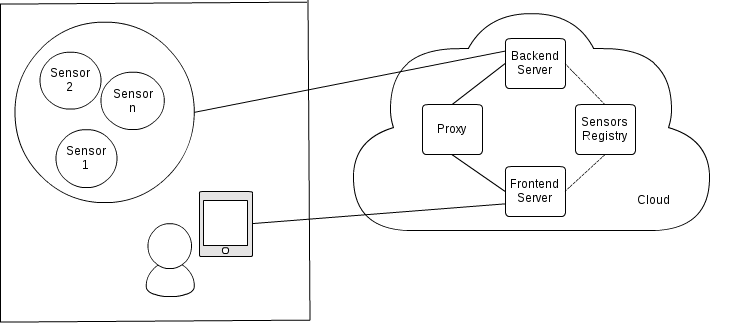
\includegraphics[scale=0.5]{images/User_Case.png}   
        \caption[Use Case]{Use Case}
        \label{img:structure}                           
        \end{figure}

\section{Application Tier}
  This layer coordinates the application, processes commands, makes logical decisions and evaluations, and performs calculations. It also moves and processes data between the two surrounding layers.
  \newline
  Application tier consists all logical modules as: Web server, Sensor registry, Proxy and Web-based Frontend. All these modules connects to each other as shown on a Figure 4.4. Detailed information about functionality of every module described in sections above.
    \begin{figure}[!ht]
    \centering
    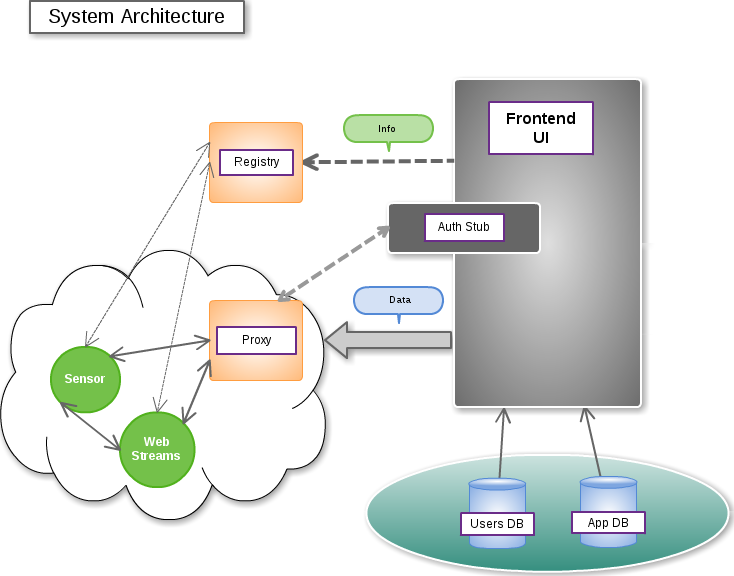
\includegraphics[scale=0.5]{images/Structure.png}   
    \caption[System Architecture]{System Architecture}
    \label{img:structure}                           
    \end{figure}

	\subsection{Web server}
  The primary function of a web server is to deliver web pages to clients. The communication between client and server takes place using the Hypertext Transfer Protocol (HTTP). Pages delivered are most frequently HTML documents, which may include images, style sheets and scripts in addition to text content. 
  \newline In proposed concept Web server responsible for dynamic distribution of tasks between various modules of common system to serve efficiently static files. Such specific operation logic like authentication of user, registration of sensors and users are delegated to an external components such as Registry, Proxy and Frontend. these external components can be interchange without dependency to the system itself.

	\subsection{Sensor Registry}
  Sensor Registry is a module responsible for keeping all required metadata of available sensors, for connecting arbitrary sensors. Frontend gets info from Registry about registered sensors and their availability. By using simple RESTful API, so that any Registry that implements suggested API and returns valid JSON, which consits such info as: id of sensor, availability(true or false), SLA, necessary bandwidth for retrieving data, title and type. By using RESTful API, the concept provides a possibility to dynamically connect and disconnect different Registries, that are required in a different context of usage. 

	\subsection{Proxy}
  Since concept of generic frontend is meant to support any type of sensor, regardless of its interface, Proxy is responsible for mapping interface of particular sensors data stream into JSOn message, delivered through XMPP protocol. Requirements to Proxy are:
  \begin{itemize}
  \item convert sensor data into particular JSON supporting scheme(specification*)
  \item implement XMPP protocol to provide exchange message with XMPP server
  \item get and parse sensor data
  \end{itemize}
    \begin{figure}[!ht]
    \centering
    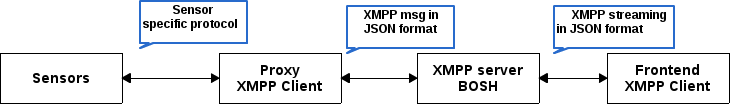
\includegraphics[scale=0.6]{images/Protocol_flow.png}   
    \caption[Protocol flow]{Protocol flow}
    \label{img:protocol}                           
    \end{figure}

  \subsection{Web-based Frontend}
    \subsubsection{Interfaces}
    According to RESTful API and simple structure of registry data, communication between Frontend and Registry will done by using HTTP get request and JSON format.
    \newline
    According to requirements to retrieve streaming data from the sensors, it is necessary to use XMPP protocol\cite{XMPPbook}.
    XMPP powers a wide range of applications including instant messaging, multi-user chat, voice and video conferencing, collaborative spaces, real-time gaming, data synchronization, and even search. Although XMPP started its life as an open, standardized alternative to proprietary instant messaging systems like ICQ and AOL Instant Messenger, it has matured into an extremely robust protocol for all kinds of exciting creations.
    \newline
    The core of XMPP is the exchange of small, structured chunks of information. Like HTTP, XMPP is a client-server protocol, but it differs from HTTP by allowing either side to send data to the other asynchronously. XMPP connections are long lived, and data is pushed instead of pulled. Because of XMPP’s differences, it provides an excellent companion protocol to HTTP. XMPP-powered web applications are to AJAX what AJAX was to the static web site; they are the next level of interactivity and dynamism. Where JavaScript and dynamic HTML have brought desktop application features to the web browser, XMPP brings new communications possibilities to the Web. XMPP has many common social web features built in, due to its instant messaging heritage. Contact lists and subscriptions create social graphs, presence updates help users keep track of who is doing what, and private messaging makes communication among users trivial. XMPP also has nearly 300 extensions, providing a broad and useful range of tools on which to build sophisticated applications. 
    \newline
    XMPP, like all protocols, defines a format for moving data between two or more communicating entities. In XMPP’s case, the entities are normally a client and a server, although it also allows for peer-to-peer communication between two servers or two clients. Many XMPP servers exist on the Internet, accessible to all, and form a federated network of interconnected systems. Data exchanged over XMPP is in XML, giving the communication a rich, extensible structure. Many modern protocols forgo the bandwidth savings of a binary encoding for the more practical feature of being human readable and therefore easily debugged. XMPP’s choice to piggyback on XML means that it can take advantage of the large amount of knowledge and supporting software for dealing with XML. One major feature XMPP gets by using XML is XML’s insensibility. It is extremely easy to add new features to the protocol that are both backward and forward compatible. This extensibility is put to great use in the more than 200 protocol extensions registered with the XMPP Standards Foundation and has provided developers with a rich and practically unlimited set of tools. XML is known primarily as a document format, but in XMPP, XML data is organized as a pair of streams, one stream for each direction of communication. Each XML stream consists of an opening element, followed by XMPP stanzas and other top-level elements, and then a closing element. Each XMPP stanza is a first-level child element of the stream with all its descendant elements and attributes. At the end of an XMPP connection, the two streams form a pair of valid XML documents.
    The Extensible Messaging and Presence Protocol (XMPP) is the IETF’s formalization of the base XML streaming protocols for instant messaging and presence developed within the Jabber community starting in 1999. This page provides a brief chronology of Jabber/XMPP technologies from the perspective of standardization\cite{xmpp}.
    \begin{itemize}
      \item \emph{Decentralization}
      \newline
      The architecture of the XMPP network is similar to email; anyone can run their own XMPP server and there is no central master server.
      \newline
      \item \emph{Open standards}
      \newline
      The Internet Engineering Task Force has formalized XMPP as an approved instant messaging and presence technology under the name of XMPP (the latest specifications are RFC 6120 and RFC 6121). No royalties are required to implement support of these specifications and their development is not tied to a single vendor.
      \newline
      \item \emph{History}
      \newline
      XMPP technologies have been in use since 1999. Multiple implementations of the XMPP standards exist for clients, servers, components, and code libraries.
      \newline
      \item \emph{Security}
      \newline
      XMPP servers can be isolated from the public XMPP network (e.g., on a company intranet), and strong security (via SASL and TLS) has been built into the core XMPP specifications.
      \newline
      \item \emph{Flexibility}
      \newline
      Custom functionality can be built on top of XMPP; to maintain interoperability, common extensions are managed by the XMPP Standards Foundation. XMPP applications beyond IM include groupchat, network management, content syndication, collaboration tools, file sharing, gaming, remote systems control and monitoring, geolocation, middleware and cloud computing, VoIP and Identity services.
      \end{itemize}
      The XMPP network uses a client–server architecture (clients do not talk directly to one another). However, it is decentralized—by design, there is no central authoritative server, as there is with services such as AOL Instant Messenger or Windows Live Messenger. Some confusion often arises on this point as there is a public XMPP server being run at jabber.org, to which a large number of users subscribe. However, anyone may run their own XMPP server on their own domain.
      Every user on the network has a unique Jabber ID (usually abbreviated as JID). To avoid requiring a central server to maintain a list of IDs, the JID is structured like an email address with a username and a domain name (or IP address[16]) for the server where that user resides, separated by an at sign (@), such as username@example.com.
    \subsubsection{Authentication Stub}

\begin{figure}[!ht]
\centering
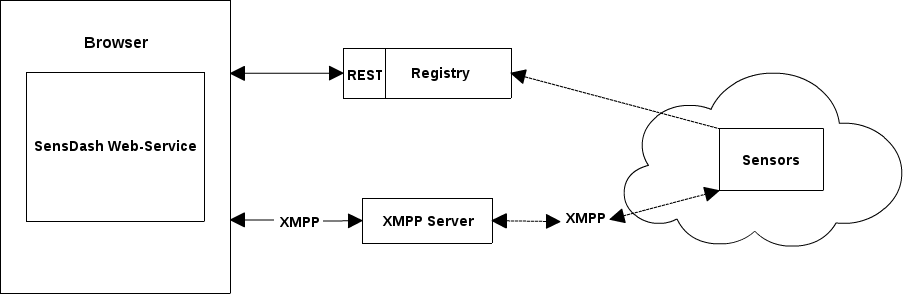
\includegraphics[scale=0.5]{images/Interface.png}   
\caption[Interface]{Interface}
\label{img:interfaces}                           
\end{figure}

\section{Data Tier}
   As was mentioned in section 4.1 Data Tier consists source of data that have to be retrieved by application tier to a client tier. Where is source of data is a data provided by sensors, in a specific type by using specific protocol, that will be handled by Application Tier. The main focus of this section determine possible characteristics of streamed data that can be retrieved by Client Tier in a lightweight scenario for mobile devices.
   \newline
    Streaming media is multimedia that is constantly received by and presented to an end-user while being delivered by a provider. Its verb form, "to stream", refers to the process of delivering media in this manner; the term refers to the delivery method of the medium rather than the medium itself. In general, media files can be delivered in one of three ways, via streaming, progressive download, or adaptive bitrate streaming.  Each has its purpose.
  \newline
    Streaming involves delivering the media to the client via a server process using specific streaming protocols (such as XMPP).  Video playing begins almost immediately, especially if the video file was encoded at a data rate similar to the effective bandwidth of the target viewer.  Streaming video is also often not cached by the client so a local copy of the video is not held in its entirety on the client machine.  While it is not impossible for an enterprising person to capture and hold a copy of the stream, it takes more effort than the casual viewer may be willing to take on.  To adapt for the slowest common denominator in regard to end-user bandwidth, streaming videos are often encoded at lower quality and data rates.
  \newline
    Progressive download simply delivers a media file via traditional web server technologies.  The file begins playing on the client as soon as enough data has been buffered to provide a smooth uninterrupted viewing experience.  Progressive downloaded files are easier to capture since an entire copy of the file is downloaded to the local device.  Also, the quality of the file can be higher simply because a user on a slower connection will just have to wait longer for the viewing to begin.
  \newline
    Adaptive bitrate streaming is a kind of best of both worlds.  As the name implies, adaptive bitrate is a streaming technology and generally requires a dedicated streaming server.  In this case, media files are transcoded into multiple bitrates with the appropriate streaming being delivered to the user based on their available bandwidth.  Adaptive streaming servers can also dynamically change the bitrate as network conditions dictate\cite{ilias2013study}.
  \newline
  This explanation shows that adaptive bitrate streaming is the most valuable and suitable for concept of a generic frontend.
  But it is necessary to go deeply in details to define limits and understanding of "good quality", "bad quality", "excellent quality".
  All three delivery methods are forms of Adaptive Bit Rate Streaming. This delivery method will have a massive impact on every aspect of Internet video delivery because it allows the stream to actually adapt the video experience to the quality of the network and the device's CPU.
  \newline
  In other words, the video stream can increase or decrease the bit rate and resolution of the video (its quality) in real time so that it’s always streaming the best possible quality the available network connection can support. The better the network connection, the better the video image quality. The fact that the stream handles all of this complexity means the mobile video viewer doesn’t have to do anything; everything is left to the stream and the player.
  \newline
  So how does this all work? To prep your video content for HLS, you start off with a high quality version of your video and encode multiple copies of it using MPEG-4 H.264. These copies are at various bit rates and resolutions ranging from lower quality renditions appropriate for slower 3G connections, up to extremely high quality renditions suitable for fast devices on fast networks. The renditions are then wrapped into MPEG-2 Transport Streams and chopped up into 10 second segments or chunks. It’s these segments that are eventually streamed to an HTML5 Video Player on a mobile device, browser or set-top box, and because the player receives the video in 10 second chunks and can detect the quality of the network connection, it can switch to a higher or lower quality video segment every ten seconds if bandwidth conditions change.
  \newline
  Mobile platform such as iOS/Mobile Encoding supports at least two video types: 3GP + MPEG-4 for less sophisticated devices, and H.264 + MP4 for smartphones. One output video can cover all of smartphone users – iPhone/iPad/iPod, Android, and (for the most part) Blackberry too. Toss in PSP, PS3, and Xbox 360 for good measure. Mobile devices well using a handful of standard encoding profiles. Start with the Universal Smartphone Profile for wide compatibility; add in an Advanced Smartphone Profile version for the more advanced devices; and round out mobile list with a legacy profile for widest compatibility – either our Legacy Smartphone Profile (below), or even a 3GP video for even wider compatibility. The following defaults are the starting point for these profiles. Default these settings by default, but you can replicate them easily enough in whatever encoding tool you're using. Defaults: Video: H.264, Level 3.0, Baseline profile Audio: AAC, 1-2 channels
  %- data on demand%
  %Your model of data streams should consider that some streams can be replayed
%and some cannot because they contain live data. Also, some may be adaptive,

\section{Summary}
	In this chapter, a first web-based concept for sensor streaming services is to be created. Along with it, a light-weight scenario service registry will be needed. Users should be able to explore not just services, but also the information provided by them, and eventually be led to advanced usage patterns such as the development of third-party applications to access the information data and real-time streams.
  \newline
  Proxy responsibilities:
  \begin{itemize}
  \item 1
  \item 2
  \item 3
  \end{itemize}
  Registry responsibilities:
  \begin{itemize}
  \item 1
  \item 2
  \item 3
  \end{itemize}
  Web-server responsibilities:
  \begin{itemize}
  \item 1
  \item 2
  \item 3
  \end{itemize}
  Frontend responsibilities:
  \begin{itemize}
  \item 1
  \item 2
  \item 3
  \end{itemize}